\documentclass[10pt,a4paper]{article}
\usepackage[margin=1.7cm]{geometry}
\usepackage{amsmath,amssymb,bm,booktabs,graphicx}
\usepackage{lmodern}
\usepackage{float}
\usepackage{placeins}
\usepackage[colorlinks=true,linkcolor=blue,citecolor=blue]{hyperref}
\usepackage[capitalize]{cleveref}
\newcommand{\bs}{\boldsymbol}
\newcommand{\dt}{\Delta t}
\newcommand{\curl}{\operatorname{curl}}
\renewcommand{\div}{\operatorname{div}}
\let\standardfigure\figure
\let\endstandardfigure\endfigure
\renewenvironment{figure}[1][]{\standardfigure[H]}{\endstandardfigure}
\begin{document}
\setcounter{section}{5}
\section{Numerical experiments}
\label{sec:numerical-experiments}
We first collect the convergence and unforced energy-dissipation
experiments for both time discretizations, and then present two
magnetically forced channel-flow applications of the second-order scheme.

\subsection{Experimental setup}
\label{subsec:experiment-setup}
We assess both time discretizations by a manufactured-solution test
on $\Omega=(0,1)^3$ with $T=2$. Each Cartesian partition into
$K\times K\times K$ cubes is subdivided into tetrahedra, with
$K=4,8,16,32$ and $\dt=1/K=h/\sqrt{3}$, where $h$ is the maximum
tetrahedron diameter. Space and time are refined together;
this experiment does not isolate the temporal convergence order.

\paragraph{Manufactured solution.}
Define
\[
q(s)=64s^3(1-s)^3,\qquad
B(x,y,z)=q(x)q(y)q(z),\qquad
S(x,y,z)=\sin^2(\pi x)\sin^2(\pi y)\sin^2(\pi z),
\]
and let $a=(1,2,3)^\intercal$, $b=(1,-1,1/2)^\intercal$, and
$c=(1,2,-1)^\intercal$. The prescribed fields are
\begin{align*}
\bs u&=\frac{1+0.1t}{C_u}\,\nabla B\times a,
&\bs\omega&=\frac{1-0.05t}{C_\omega}\,B b,
&\bs m&=\frac{1+0.05t}{C_m}\,S c,\\
\varphi&=\frac{1-0.05t}{C_\varphi}\,B,
&\bs H&=\nabla\varphi,
&p&=\frac{1+0.05t}{C_p}\prod_{s\in\{x,y,z\}}\cos(2\pi s),
\end{align*}
where the fixed normalization constants used in the computations are
\begin{gather*}
C_u=363.275188821,\quad C_\omega=20.6500992827,\quad
C_m=\frac{\sqrt{81+108\pi^2}}{16},\\
C_\varphi=13.7667328551,\qquad C_p=0.353553390593.
\end{gather*}
The auxiliary fields are $\bs k=\curl\bs m$, $\bs z=\bs u\times\bs m$,
$\vartheta=-\Delta\varphi$, and $\varpi=\bs u\cdot\bs m$.
We set $\bs H_e=-\mu_0(\bs m+\bs H)$ and use the zero-mean modified
pressure $\widetilde p=\mathcal P_0[p-\mu_0\bs m\cdot\bs H/2]$, where
$\mathcal P_0v=v-|\Omega|^{-1}\int_\Omega v$.
All physical parameters $\rho,\kappa,\eta,\zeta,\mu_0,\sigma,
\eta^\prime,\lambda^\prime,\tau,\chi_0$ are set to one.

This is a forced verification problem. The momentum, angular-momentum,
and magnetization sources $\bs f,\bs g,\bs r$ are obtained by substituting
the prescribed fields into the corresponding continuous equations.
Their weak right-hand sides are $(\bs f,\bs v_h)$,
$(\bs g,\bs s_h)$, and $(\bs r,\bs F_h)$; the magnetic-potential
right-hand side is
\[
\left(-\partial_t\bs H_e
-\frac{\mu_0+\chi_0}{\tau\mu_0}\bs H_e
+\sigma\nabla\div\bs H_e-\mu_0\bs r,\nabla\psi_h\right).
\]
The fields satisfy the homogeneous boundary traces used in the experiment:
zero velocity and angular velocity, zero normal magnetization,
zero tangential $\bs z,\bs k,\bs H$, and zero
$\varphi,\vartheta,\varpi$. In particular, $q,q',q''$ vanish at both
endpoints and $S,\nabla S$ vanish on the cube boundary. The new
$\vartheta$ and $\varpi$ couplings are not identically zero for this test.

\paragraph{Discretization and implementation.}
The first-order runs use the MINI velocity element, continuous piecewise
linear pressure and angular velocity, lowest-order Raviart--Thomas
magnetization and first-family Nedelec $\bs z,\bs k,\bs H$, and
continuous piecewise linear $\varphi,\vartheta,\varpi$.

For the second-order scheme, velocity and angular velocity use continuous
piecewise quadratic elements, pressure remains continuous piecewise linear, magnetization
uses RT1, and $\bs z,\bs k,\bs H$ use first-family Nedelec elements
one degree above the lowest order. The scalar fields
$\varphi,\vartheta,\varpi$ are continuous piecewise quadratic.
The corresponding RT and Nedelec Basix degree is two.

The initial velocity is obtained by a discrete Stokes projection.
After interpolating the initial magnetization into its RT space,
the initial potential is determined from the compatible magnetic Poisson
problem. The initial $\bs k,\bs z,\vartheta,\varpi$ satisfy their discrete
mass-projection relations. Pressure is normalized by its finite-element
integral mean.

For the second-order convergence test, the first time step is solved
by a Broyden quasi-Newton iteration with
relative tolerance $10^{-9}$ and a maximum of 12 iterations.
The accepted state is checked by reassembling the nonlinear midpoint
equations. Subsequent time steps use the prescribed extrapolated
coefficients and require one five-block linear solve per step.
The $\bs z_h$ and $\varpi_h$ slots represent the current midpoint-stage
projections; they are not averaged again with the preceding stage.

Computations use FEniCSx/DOLFINx~0.10.0~\cite{Barattafenics}
with PETSc and MUMPS. The five-block Algorithm~3 is evaluated through
matrix-free Schur-complement actions. The $K_1,K_3,K_5$ subproblems use
MUMPS LU; the $S_2,S_4$ systems use FGMRES with LU preconditioners.
The MUMPS ordering control is $\mathrm{ICNTL}(7)=7$.
The Schur tolerances are $10^{-10}$ relative and $10^{-12}$ absolute.
All first-order cases and the second-order cases up to $K=16$ use
48 MPI processes with one thread each; the second-order $K=32$ case
uses 32 MPI processes with four threads each on a 1-TB-class node.
Source terms are evaluated at quadrature points, with assembly
quadrature degree 12. In the error calculations, the analytic values
and derivatives are independently represented in a degree-6 DG space
and integrated with degree-12 quadrature; the numerical solution is
evaluated in its original finite-element space.

As implementation checks for the manufactured-solution runs,
the two schemes were compared with a
monolithic solve of the same matrix at the first two time levels on
$K=4$, modulo the same pressure
nullspace; the normalized solution differences were below $1.1\times10^{-12}$.
An independent transcription of the nine weak equations on $K=2$,
using random finite-element fields and both unit and non-unit parameters,
also agreed with the production matrices and right-hand sides to
scaled differences below $1.1\times10^{-16}$.
These checks concern algebraic and implementation consistency, rather
than replacing the convergence test.

\paragraph{Error measures.}
For a field $v$ and its specified norm $X$, we report
\[
E_X(v)=\frac{\|v-v_h\|_X}{\|v\|_X},\qquad
\mathrm{rate}(K\to2K)=\log_2\frac{E_X(v;K)}{E_X(v;2K)}.
\]
The norms are full $H^1$ for $\bs u,\bs\omega,\varphi$, $L^2$ for
$\widetilde p,\bs k$, $H(\div)$ for $\bs m$, and $H(\curl)$ for
$\bs H$. Thus the graph norms combine the squared $L^2$ and derivative
terms before taking the square root. Pressure errors use zero-mean
numerical and exact fields. First-order errors are evaluated at $T$.

For the second-order scheme, the primary fields are compared at $T$.
Its pressure slot represents the averaged modified pressure, so its reference is
\[
\widetilde p_{\mathrm{ref}}^{N-1/2}
=\frac{\widetilde p(T)+\widetilde p(T-\dt)}{2},
\]
with the same zero-mean convention as above. This reference is not
identified with either the endpoint pressure or the analytic pressure
evaluated directly at the midpoint.

We also report $C_H$, the maximum of $|\curl\bs H_h|$ over the
degree-6 DG interpolation points, as a sampled estimate of
$\|\curl\bs H_h\|_{L^\infty}$. It is an absolute diagnostic, not a
relative error or a rigorous continuous supremum.


\subsection{Convergence verification}
\label{subsec:convergence-verification}
We report the joint space--time refinement results separately for the
two schemes, using the common test and error measures defined above.
\subsection{Numerical experiments}
\label{subsec:revised-numerical-first}
We assess the first-order discretization by a manufactured-solution test
on $\Omega=(0,1)^3$ with $T=2$. Each Cartesian partition into
$K\times K\times K$ cubes is subdivided into tetrahedra, with
$K=4,8,16,32$ and $\dt=1/K=h/\sqrt{3}$, where $h$ is the maximum
tetrahedron diameter. The same test is used for the second-order scheme
below. Space and time are refined together; this experiment does not
isolate the temporal convergence order.

\paragraph{Manufactured solution.}
Define
\[
q(s)=64s^3(1-s)^3,\qquad
B(x,y,z)=q(x)q(y)q(z),\qquad
S(x,y,z)=\sin^2(\pi x)\sin^2(\pi y)\sin^2(\pi z),
\]
and let $a=(1,2,3)^\intercal$, $b=(1,-1,1/2)^\intercal$, and
$c=(1,2,-1)^\intercal$. The prescribed fields are
\begin{align*}
\bs u&=\frac{1+0.1t}{C_u}\,\nabla B\times a,
&\bs\omega&=\frac{1-0.05t}{C_\omega}\,B b,
&\bs m&=\frac{1+0.05t}{C_m}\,S c,\\
\varphi&=\frac{1-0.05t}{C_\varphi}\,B,
&\bs H&=\nabla\varphi,
&p&=\frac{1+0.05t}{C_p}\prod_{s\in\{x,y,z\}}\cos(2\pi s),
\end{align*}
where the fixed normalization constants used in the computations are
\begin{gather*}
C_u=363.275188821,\quad C_\omega=20.6500992827,\quad
C_m=\frac{\sqrt{81+108\pi^2}}{16},\\
C_\varphi=13.7667328551,\qquad C_p=0.353553390593.
\end{gather*}
The auxiliary fields are $\bs k=\curl\bs m$, $\bs z=\bs u\times\bs m$,
$\vartheta=-\Delta\varphi$, and $\varpi=\bs u\cdot\bs m$.
We set $\bs H_e=-\mu_0(\bs m+\bs H)$ and use the zero-mean modified
pressure $\widetilde p=\mathcal P_0[p-\mu_0\bs m\cdot\bs H/2]$, where
$\mathcal P_0v=v-|\Omega|^{-1}\int_\Omega v$.
All physical parameters $\rho,\kappa,\eta,\zeta,\mu_0,\sigma,
\eta^\prime,\lambda^\prime,\tau,\chi_0$ are set to one.

This is a forced verification problem. The momentum, angular-momentum,
and magnetization sources $\bs f,\bs g,\bs r$ are obtained by substituting
the prescribed fields into the corresponding continuous equations.
Their weak right-hand sides are $(\bs f,\bs v_h)$,
$(\bs g,\bs s_h)$, and $(\bs r,\bs F_h)$; the magnetic-potential
right-hand side is
\[
\left(-\partial_t\bs H_e
-\frac{\mu_0+\chi_0}{\tau\mu_0}\bs H_e
+\sigma\nabla\div\bs H_e-\mu_0\bs r,\nabla\psi_h\right).
\]
The fields satisfy the homogeneous boundary traces used in the experiment:
zero velocity and angular velocity, zero normal magnetization,
zero tangential $\bs z,\bs k,\bs H$, and zero
$\varphi,\vartheta,\varpi$. In particular, $q,q',q''$ vanish at both
endpoints and $S,\nabla S$ vanish on the cube boundary. The new
$\vartheta$ and $\varpi$ couplings are not identically zero for this test.

\paragraph{Discretization and implementation.}
The first-order runs use the MINI velocity element, continuous piecewise
linear pressure and angular velocity, lowest-order Raviart--Thomas
magnetization and first-family Nedelec $\bs z,\bs k,\bs H$, and
continuous piecewise linear $\varphi,\vartheta,\varpi$.
The initial velocity is obtained by a discrete Stokes projection.
After interpolating the initial magnetization into its RT space,
the initial potential is determined from the compatible magnetic Poisson
problem. The initial $\bs k,\bs z,\vartheta,\varpi$ satisfy their discrete
mass-projection relations. Pressure is normalized by its finite-element
integral mean.

Computations use FEniCSx/DOLFINx~0.10.0~\cite{Barattafenics}
with PETSc and MUMPS. The five-block Algorithm~3 is evaluated through
matrix-free Schur-complement actions. The $K_1,K_3,K_5$ subproblems use
MUMPS LU; the $S_2,S_4$ systems use FGMRES with LU preconditioners.
The MUMPS ordering control is $\mathrm{ICNTL}(7)=7$.
The Schur tolerances are $10^{-10}$ relative and $10^{-12}$ absolute.
All first-order cases and the second-order cases up to $K=16$ use
48 MPI processes with one thread each; the second-order $K=32$ case
uses 32 MPI processes with four threads each on a 1-TB-class node.
Source terms are evaluated at quadrature points, with assembly
quadrature degree 12. In the error calculations, the analytic values
and derivatives are independently represented in a degree-6 DG space
and integrated with degree-12 quadrature; the numerical solution is
evaluated in its original finite-element space.

As implementation checks, the two schemes were compared with a
monolithic solve of the same matrix at the first two time levels on
$K=4$, modulo the same pressure
nullspace; the normalized solution differences were below $1.1\times10^{-12}$.
An independent transcription of the nine weak equations on $K=2$,
using random finite-element fields and both unit and non-unit parameters,
also agreed with the production matrices and right-hand sides to
scaled differences below $1.1\times10^{-16}$.
These checks concern algebraic and implementation consistency, rather
than replacing the convergence test.

\paragraph{Error measures.}
For a field $v$ and its specified norm $X$, we report
\[
E_X(v)=\frac{\|v-v_h\|_X}{\|v\|_X},\qquad
\mathrm{rate}(K\to2K)=\log_2\frac{E_X(v;K)}{E_X(v;2K)}.
\]
The norms are full $H^1$ for $\bs u,\bs\omega,\varphi$, $L^2$ for
$\widetilde p,\bs k$, $H(\div)$ for $\bs m$, and $H(\curl)$ for
$\bs H$. Thus the graph norms combine the squared $L^2$ and derivative
terms before taking the square root. Pressure errors use zero-mean
numerical and exact fields. First-order errors are evaluated at $T$.
We also report $C_H$, the maximum of $|\curl\bs H_h|$ over the
degree-6 DG interpolation points, as a sampled estimate of
$\|\curl\bs H_h\|_{L^\infty}$. It is an absolute diagnostic, not a
relative error or a rigorous continuous supremum.

\paragraph{First-order results.}
\Cref{tab:first-order-errors} gives the errors and observed orders;
\Cref{fig:first-order-convergence-rates} shows the corresponding
log--log error curves. On the finest refinement interval, the rates
for $\bs u,\bs\omega,\bs m,\bs k,\varphi,\bs H$ are
1.019, 0.994, 0.999, 0.997, 1.018, and 1.017, respectively.
The modified pressure exhibits a rate of 2.065 in this test.
The sampled curl diagnostic remains between $1.22\times10^{-13}$
and $8.51\times10^{-12}$, consistent with the discrete gradient
recovery of the magnetic field up to numerical error.

\begin{table}[htbp]
\centering
\caption{Relative errors and observed rates for the first-order scheme, $T=2$ and $\dt=1/K$. $C_H$ is the sampled absolute curl diagnostic.}
\label{tab:first-order-errors}
\begingroup
\small
\setlength{\tabcolsep}{3.5pt}
\renewcommand{\arraystretch}{1.15}
\begin{tabular}{crrrrrrrr}
\toprule
\multicolumn{9}{c}{(a) Velocity, pressure, angular velocity, and magnetization}\\
\midrule
$K$ & \multicolumn{2}{c}{$\bs u$: $H^1$} & \multicolumn{2}{c}{$\widetilde p$: $L^2$} & \multicolumn{2}{c}{$\bs\omega$: $H^1$} & \multicolumn{2}{c}{$\bs m$: $H(\div)$}\\
 & Error & Rate & Error & Rate & Error & Rate & Error & Rate\\
\midrule
4 & $9.6554\!\times\!10^{-1}$ & -- & $5.6019\!\times\!10^{-1}$ & -- & $6.4182\!\times\!10^{-1}$ & -- & $3.9160\!\times\!10^{-1}$ & --\\
8 & $4.3070\!\times\!10^{-1}$ & 1.165 & $1.0260\!\times\!10^{-1}$ & 2.449 & $3.5671\!\times\!10^{-1}$ & 0.847 & $1.9873\!\times\!10^{-1}$ & 0.979\\
16 & $1.9858\!\times\!10^{-1}$ & 1.117 & $2.1172\!\times\!10^{-2}$ & 2.277 & $1.8331\!\times\!10^{-1}$ & 0.960 & $9.9738\!\times\!10^{-2}$ & 0.995\\
32 & $9.8002\!\times\!10^{-2}$ & 1.019 & $5.0596\!\times\!10^{-3}$ & 2.065 & $9.2018\!\times\!10^{-2}$ & 0.994 & $4.9919\!\times\!10^{-2}$ & 0.999\\
\bottomrule
\end{tabular}
\par\medskip
\begin{tabular}{crrrrrrr}
\toprule
\multicolumn{8}{c}{(b) Auxiliary curl field, potential, magnetic field, and curl diagnostic}\\
\midrule
$K$ & \multicolumn{2}{c}{$\bs k$: $L^2$} & \multicolumn{2}{c}{$\varphi$: $H^1$} & \multicolumn{2}{c}{$\bs H$: $H(\curl)$} & $C_H$\\
 & Error & Rate & Error & Rate & Error & Rate &\\
\midrule
4 & $5.1511\!\times\!10^{-1}$ & -- & $6.5848\!\times\!10^{-1}$ & -- & $6.6223\!\times\!10^{-1}$ & -- & $1.2220\!\times\!10^{-13}$\\
8 & $2.6813\!\times\!10^{-1}$ & 0.942 & $3.7678\!\times\!10^{-1}$ & 0.805 & $3.7965\!\times\!10^{-1}$ & 0.803 & $5.1946\!\times\!10^{-13}$\\
16 & $1.3523\!\times\!10^{-1}$ & 0.988 & $1.8757\!\times\!10^{-1}$ & 1.006 & $1.8935\!\times\!10^{-1}$ & 1.004 & $2.0267\!\times\!10^{-12}$\\
32 & $6.7750\!\times\!10^{-2}$ & 0.997 & $9.2620\!\times\!10^{-2}$ & 1.018 & $9.3572\!\times\!10^{-2}$ & 1.017 & $8.5067\!\times\!10^{-12}$\\
\bottomrule
\end{tabular}
\endgroup
\end{table}

\begin{figure}[htbp]
\centering
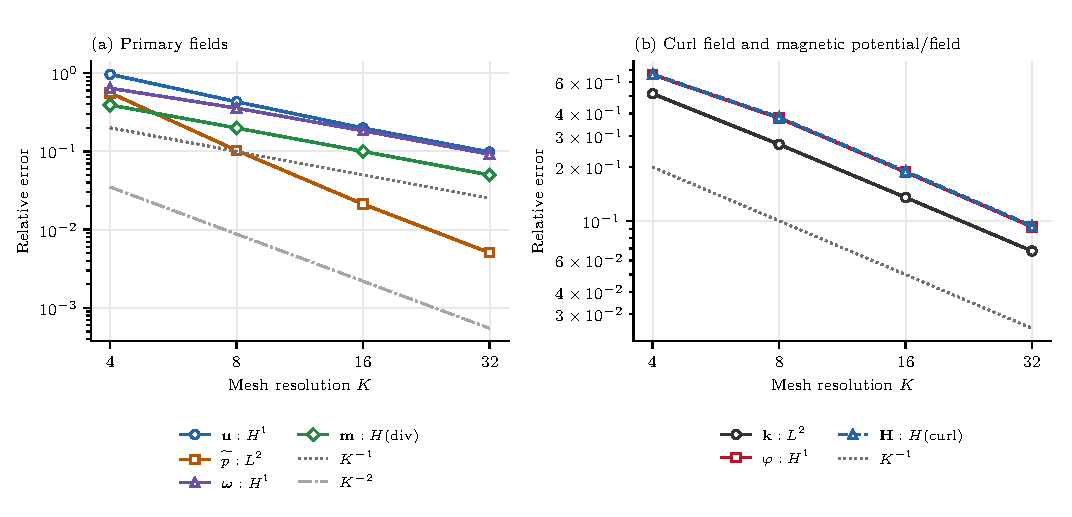
\includegraphics[width=\textwidth]{figures/first_order_errors.pdf}
\caption{Relative errors for the first-order discretization under joint
refinement with $\dt=1/K$.
(a) Velocity, modified pressure, angular velocity, and magnetization.
(b) Auxiliary curl field, magnetic potential, and magnetic field.
The horizontal coordinate is the mesh resolution $K=4,8,16,32$, so
refinement proceeds from left to right. Reference lines proportional
to $K^{-1}$ and $K^{-2}$ indicate first- and second-order decay with
mesh refinement, not independently measured temporal orders.}
\label{fig:first-order-convergence-rates}
\end{figure}

\FloatBarrier
\paragraph{Unforced energy dissipation.}
We next test free relaxation on the fixed $K=8$ mesh, with $T=0.5$
and $\dt=1/16,1/32,1/64$. All physical parameters remain one.
Unlike the manufactured-solution test, the applied field and all
compensating sources are set to zero:
$\bs H_e=\bs f=\bs g=\bs r=0$.
We retain the homogeneous boundary traces described above.
The initial shapes are
\[
\bs u_0=C_u^{-1}\nabla B\times a,\qquad
\bs\omega_0=C_\omega^{-1}B b,\qquad
\bs m_0=C_m^{-1}S c.
\]
The initial velocity is projected onto the discrete solenoidal space;
angular velocity and magnetization are interpolated into their
respective spaces. The initial potential is recomputed with zero
boundary trace from
\[
(\nabla\varphi_h^0,\nabla\psi_h)
=-(\bs m_h^0,\nabla\psi_h)
\qquad\text{for all admissible }\psi_h,
\]
rather than prescribed from the manufactured magnetic potential.
The auxiliary variables satisfy their discrete projection relations.
Thus the internal magnetic field is not artificially suppressed,
and the subsequent solution is not constrained to follow the
manufactured temporal profile.

At every time level we integrate the discrete energy
\begin{equation}\label{eq:energy-test-observable}
E_h^n=\frac12\left(
\rho\|\bs u_h^n\|^2+
\rho\kappa\|\bs\omega_h^n\|^2+
\|\bs m_h^n\|^2+
\mu_0\|\nabla\varphi_h^n\|^2\right).
\end{equation}
The norms in \eqref{eq:energy-test-observable} are spatial $L^2$ norms.
Energy and dissipation are evaluated in the original finite-element
spaces using degree-12 quadrature, not from the visualization fields.
We also check the balance defect
\begin{equation}\label{eq:energy-test-first-balance}
R_h^n=E_h^n-E_h^{n-1}+\dt D_h^n+N_h^n,
\qquad
N_h^n=\tfrac12\|\mathcal X_h^n-\mathcal X_h^{n-1}\|_{\mathtt D}^2,
\end{equation}
where $D_h^n$ is the discrete viscous, spin, magnetic-diffusion,
and relaxation dissipation corresponding to $\mathtt A$.
In particular, the weak magnetic diffusion terms are evaluated as
$\sigma\|\bs k_h^n\|^2$ and
$\sigma\mu_0\|\vartheta_h^n\|^2$.
For both schemes, the reported balance diagnostic is
\[
\epsilon_{\rm bal}^n=
\frac{|R_h^n|}{\max\{E_h^n,E_h^{n-1},\dt D_h^n+N_h^n,
10^{-14}E_h^0\}},
\]
with the midpoint dissipation and $N_h^n=0$ used for the
second-order scheme.

All energy runs use 48 MPI processes with one thread each and the
same five-block solver settings as the convergence experiments.
The first-order runs require no nonlinear startup.
\Cref{fig:first-order-energy} shows monotone decay for all three
time steps. The initial discrete energy is approximately
$4.205865\times10^{-2}$; the final energy ratios and balance
diagnostics are given in \Cref{tab:first-order-energy}.
The largest balance diagnostic is $4.61\times10^{-14}$.
These results verify dissipation for the tested discretizations;
they do not constitute a pure temporal convergence study.

\begin{table}[htbp]
\centering
\caption{First-order unforced energy test: $K=8$, $T=0.5$.}
\label{tab:first-order-energy}
\small
\begin{tabular}{crr}
\toprule
$\dt$ & $E_h(T)/E_h(0)$ & $\max_n\epsilon_{\rm bal}^n$\\
\midrule
$1/16$ & $9.1847\times10^{-5}$ & $3.69\times10^{-14}$\\
$1/32$ & $3.1955\times10^{-5}$ & $2.22\times10^{-14}$\\
$1/64$ & $1.6247\times10^{-5}$ & $4.61\times10^{-14}$\\
\bottomrule
\end{tabular}
\end{table}

\begin{figure}[htbp]
\centering
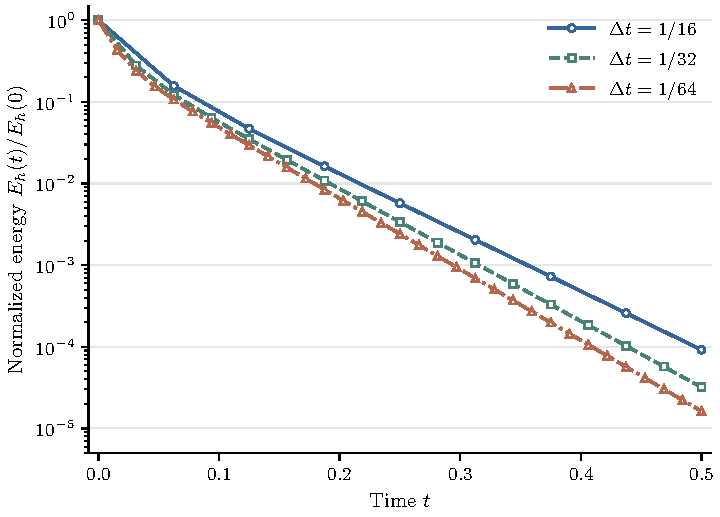
\includegraphics[width=0.70\textwidth]{figures/first_order_energy.pdf}
\caption{Normalized discrete energy for the first-order scheme in the
unforced relaxation test, $K=8$ and $T=0.5$.
The vertical axis is logarithmic. Symbols represent all computed time
levels; connecting lines are not fitted or smoothed curves.
The same discrete initial state is used for all three time steps.}
\label{fig:first-order-energy}
\end{figure}
\FloatBarrier


\subsection{Numerical results}
\label{subsec:numerical-second-order}
We apply the second-order discretization to the same manufactured
solution, forcing, parameters, and meshes specified in
\Cref{subsec:revised-numerical-first}, retaining $T=2$ and $\dt=1/K$.
Velocity and angular velocity now use continuous piecewise quadratic
elements, pressure remains continuous piecewise linear, magnetization
uses RT1, and $\bs z,\bs k,\bs H$ use first-family Nedelec elements
one degree above the lowest order. The scalar fields
$\varphi,\vartheta,\varpi$ are continuous piecewise quadratic.
The corresponding RT and Nedelec Basix degree is two.

The first time step is solved by a Broyden quasi-Newton iteration with
relative tolerance $10^{-9}$ and a maximum of 12 iterations.
The accepted state is checked by reassembling the nonlinear midpoint
equations. Subsequent time steps use the prescribed extrapolated
coefficients and require one five-block linear solve per step.
The $\bs z_h$ and $\varpi_h$ slots represent the current midpoint-stage
projections; they are not averaged again with the preceding stage.

The primary fields are compared at $T$. The pressure slot represents
the averaged modified pressure, so its reference is
\[
\widetilde p_{\mathrm{ref}}^{N-1/2}
=\frac{\widetilde p(T)+\widetilde p(T-\dt)}{2},
\]
with the same zero-mean convention as above. This reference is not
identified with either the endpoint pressure or the analytic pressure
evaluated directly at the midpoint.

\Cref{tab:second-order-errors,fig:second-order-convergence} show that
the finest-grid rates for $\bs u,\widetilde p,\bs\omega,\bs m,
\varphi,\bs H$ are 2.166, 2.051, 1.981, 2.007, 1.968, and 1.968,
respectively. The $L^2$ error of $\bs k$ decreases approximately at
first order, with a finest-grid rate of 1.015; second-order convergence
is therefore not claimed for every auxiliary quantity.
The sampled curl diagnostic ranges from $7.30\times10^{-13}$ to
$6.96\times10^{-11}$. For $K=32$, all 64 steps reach $T=2$, and
the final full-system relative algebraic residual is
$2.08\times10^{-13}$.
These observations support the reported joint-refinement behavior.
Because the mesh and time step vary together and the primary exact
fields have linear temporal amplitudes, they do not constitute a
separate test of pure temporal accuracy or of energy stability.

\begin{table}[htbp]
\centering
\caption{Relative errors and observed rates for the second-order scheme, $T=2$ and $\dt=1/K$. $C_H$ is the sampled absolute curl diagnostic.}
\label{tab:second-order-errors}
\begingroup
\small
\setlength{\tabcolsep}{3.5pt}
\renewcommand{\arraystretch}{1.15}
\begin{tabular}{crrrrrrrr}
\toprule
\multicolumn{9}{c}{(a) Velocity, pressure, angular velocity, and magnetization}\\
\midrule
$K$ & \multicolumn{2}{c}{$\bs u$: $H^1$} & \multicolumn{2}{c}{$\widetilde p$: $L^2$} & \multicolumn{2}{c}{$\bs\omega$: $H^1$} & \multicolumn{2}{c}{$\bs m$: $H(\div)$}\\
 & Error & Rate & Error & Rate & Error & Rate & Error & Rate\\
\midrule
4 & $5.6873\!\times\!10^{-1}$ & -- & $4.2000\!\times\!10^{-1}$ & -- & $2.1381\!\times\!10^{-1}$ & -- & $1.1937\!\times\!10^{-1}$ & --\\
8 & $1.5090\!\times\!10^{-1}$ & 1.914 & $9.4815\!\times\!10^{-2}$ & 2.147 & $6.2017\!\times\!10^{-2}$ & 1.786 & $3.1613\!\times\!10^{-2}$ & 1.917\\
16 & $2.4805\!\times\!10^{-2}$ & 2.605 & $2.0872\!\times\!10^{-2}$ & 2.184 & $1.6320\!\times\!10^{-2}$ & 1.926 & $7.8383\!\times\!10^{-3}$ & 2.012\\
32 & $5.5259\!\times\!10^{-3}$ & 2.166 & $5.0382\!\times\!10^{-3}$ & 2.051 & $4.1345\!\times\!10^{-3}$ & 1.981 & $1.9494\!\times\!10^{-3}$ & 2.007\\
\bottomrule
\end{tabular}
\par\medskip
\begin{tabular}{crrrrrrr}
\toprule
\multicolumn{8}{c}{(b) Auxiliary curl field, potential, magnetic field, and curl diagnostic}\\
\midrule
$K$ & \multicolumn{2}{c}{$\bs k$: $L^2$} & \multicolumn{2}{c}{$\varphi$: $H^1$} & \multicolumn{2}{c}{$\bs H$: $H(\curl)$} & $C_H$\\
 & Error & Rate & Error & Rate & Error & Rate &\\
\midrule
4 & $2.1008\!\times\!10^{-1}$ & -- & $2.0119\!\times\!10^{-1}$ & -- & $2.0303\!\times\!10^{-1}$ & -- & $7.3001\!\times\!10^{-13}$\\
8 & $9.5804\!\times\!10^{-2}$ & 1.133 & $6.0098\!\times\!10^{-2}$ & 1.743 & $6.0718\!\times\!10^{-2}$ & 1.742 & $3.9064\!\times\!10^{-12}$\\
16 & $4.6084\!\times\!10^{-2}$ & 1.056 & $1.6119\!\times\!10^{-2}$ & 1.899 & $1.6289\!\times\!10^{-2}$ & 1.898 & $1.8492\!\times\!10^{-11}$\\
32 & $2.2804\!\times\!10^{-2}$ & 1.015 & $4.1189\!\times\!10^{-3}$ & 1.968 & $4.1627\!\times\!10^{-3}$ & 1.968 & $6.9611\!\times\!10^{-11}$\\
\bottomrule
\end{tabular}
\endgroup
\end{table}

\begin{figure}[htbp]
\centering
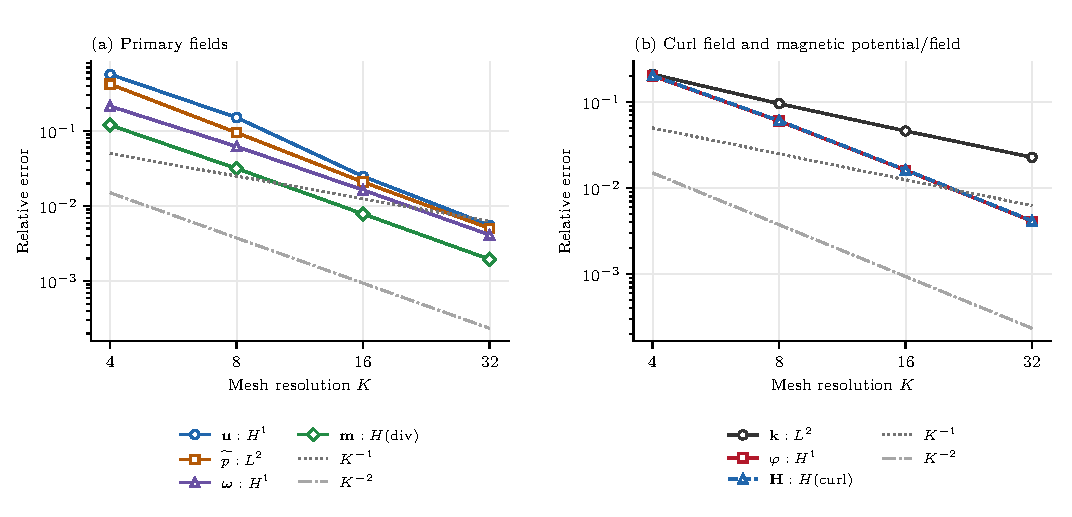
\includegraphics[width=\textwidth]{figures/second_order_errors.pdf}
\caption{Relative errors for the second-order discretization using the
same manufactured solution and $\dt=1/K$.
(a) Velocity, averaged modified pressure, angular velocity, and magnetization.
(b) Auxiliary curl field, magnetic potential, and magnetic field.
The horizontal coordinate is $K=4,8,16,32$, increasing from left to
right. Reference lines proportional to $K^{-1}$ and $K^{-2}$ distinguish
the nearly quadratic decay of the principal errors from the
approximately first-order $L^2$ decay for $\bs k$.}
\label{fig:second-order-convergence}
\end{figure}


\subsection{Energy dissipation}
\label{subsec:energy-dissipation}
We test free relaxation on the fixed $K=8$ mesh, with $T=0.5$
and $\dt=1/16,1/32,1/64$. All physical parameters remain one.
Unlike the manufactured-solution test, the applied field and all
compensating sources are set to zero:
$\bs H_e=\bs f=\bs g=\bs r=0$.
We retain the homogeneous boundary traces specified in
\Cref{subsec:experiment-setup}.
The initial shapes are
\[
\bs u_0=C_u^{-1}\nabla B\times a,\qquad
\bs\omega_0=C_\omega^{-1}B b,\qquad
\bs m_0=C_m^{-1}S c.
\]
The initial velocity is projected onto the discrete solenoidal space;
angular velocity and magnetization are interpolated into their
respective spaces. The initial potential is recomputed with zero
boundary trace from
\[
(\nabla\varphi_h^0,\nabla\psi_h)
=-(\bs m_h^0,\nabla\psi_h)
\qquad\text{for all admissible }\psi_h,
\]
rather than prescribed from the manufactured magnetic potential.
The auxiliary variables satisfy their discrete projection relations.
Thus the internal magnetic field is not artificially suppressed,
and the subsequent solution is not constrained to follow the
manufactured temporal profile.

At every time level we integrate the discrete energy
\begin{equation}\label{eq:energy-test-observable}
E_h^n=\frac12\left(
\rho\|\bs u_h^n\|^2+
\rho\kappa\|\bs\omega_h^n\|^2+
\|\bs m_h^n\|^2+
\mu_0\|\nabla\varphi_h^n\|^2\right).
\end{equation}
The norms in \eqref{eq:energy-test-observable} are spatial $L^2$ norms.
Energy and dissipation are evaluated in the original finite-element
spaces using degree-12 quadrature, not from the visualization fields.
For the first-order scheme, we check the balance defect
\begin{equation}\label{eq:energy-test-first-balance}
R_h^n=E_h^n-E_h^{n-1}+\dt D_h^n+N_h^n,
\qquad
N_h^n=\tfrac12\|\mathcal X_h^n-\mathcal X_h^{n-1}\|_{\mathtt D}^2,
\end{equation}
where $D_h^n$ is the discrete viscous, spin, magnetic-diffusion,
and relaxation dissipation corresponding to $\mathtt A$.
In particular, the weak magnetic diffusion terms are evaluated as
$\sigma\|\bs k_h^n\|^2$ and
$\sigma\mu_0\|\vartheta_h^n\|^2$.
For the second-order discretization, the balance defect is
\begin{equation}\label{eq:energy-test-second-balance}
R_h^n=E_h^n-E_h^{n-1}+\dt D_h^{n-1/2},
\end{equation}
where $D_h^{n-1/2}$ is evaluated at the midpoint averages of the
primary fields and the endpoint auxiliaries
$\bs k_h,\vartheta_h$.
There is no first-order numerical-dissipation term $N_h^n$.
The stage fields $\bs z_h,\varpi_h$ are not averaged a second time.

For both schemes, the reported balance diagnostic is
\[
\epsilon_{\rm bal}^n=
\frac{|R_h^n|}{\max\{E_h^n,E_h^{n-1},\dt D_h^n+N_h^n,
10^{-14}E_h^0\}},
\]
with the midpoint dissipation and $N_h^n=0$ used for the
second-order scheme.

Both schemes retain the spatial approximation orders specified in
\Cref{subsec:experiment-setup}. Thus their discrete initial states differ,
whereas each scheme uses the same initial state for all three time steps.

All energy runs use 48 MPI processes with one thread each and the
same five-block solver settings as the convergence experiments.
The first-order runs require no nonlinear startup.

For the second-order energy test, the initial Broyden solve uses relative tolerance
$10^{-10}$ with at most 20 iterations, and the accepted midpoint
equations are independently reassembled to check their residual.
Subsequent time steps use the prescribed extrapolation.

\FloatBarrier
\paragraph{Unforced energy dissipation.}
We next test free relaxation on the fixed $K=8$ mesh, with $T=0.5$
and $\dt=1/16,1/32,1/64$. All physical parameters remain one.
Unlike the manufactured-solution test, the applied field and all
compensating sources are set to zero:
$\bs H_e=\bs f=\bs g=\bs r=0$.
We retain the homogeneous boundary traces described above.
The initial shapes are
\[
\bs u_0=C_u^{-1}\nabla B\times a,\qquad
\bs\omega_0=C_\omega^{-1}B b,\qquad
\bs m_0=C_m^{-1}S c.
\]
The initial velocity is projected onto the discrete solenoidal space;
angular velocity and magnetization are interpolated into their
respective spaces. The initial potential is recomputed with zero
boundary trace from
\[
(\nabla\varphi_h^0,\nabla\psi_h)
=-(\bs m_h^0,\nabla\psi_h)
\qquad\text{for all admissible }\psi_h,
\]
rather than prescribed from the manufactured magnetic potential.
The auxiliary variables satisfy their discrete projection relations.
Thus the internal magnetic field is not artificially suppressed,
and the subsequent solution is not constrained to follow the
manufactured temporal profile.

At every time level we integrate the discrete energy
\begin{equation}\label{eq:energy-test-observable}
E_h^n=\frac12\left(
\rho\|\bs u_h^n\|^2+
\rho\kappa\|\bs\omega_h^n\|^2+
\|\bs m_h^n\|^2+
\mu_0\|\nabla\varphi_h^n\|^2\right).
\end{equation}
The norms in \eqref{eq:energy-test-observable} are spatial $L^2$ norms.
Energy and dissipation are evaluated in the original finite-element
spaces using degree-12 quadrature, not from the visualization fields.
We also check the balance defect
\begin{equation}\label{eq:energy-test-first-balance}
R_h^n=E_h^n-E_h^{n-1}+\dt D_h^n+N_h^n,
\qquad
N_h^n=\tfrac12\|\mathcal X_h^n-\mathcal X_h^{n-1}\|_{\mathtt D}^2,
\end{equation}
where $D_h^n$ is the discrete viscous, spin, magnetic-diffusion,
and relaxation dissipation corresponding to $\mathtt A$.
In particular, the weak magnetic diffusion terms are evaluated as
$\sigma\|\bs k_h^n\|^2$ and
$\sigma\mu_0\|\vartheta_h^n\|^2$.
For both schemes, the reported balance diagnostic is
\[
\epsilon_{\rm bal}^n=
\frac{|R_h^n|}{\max\{E_h^n,E_h^{n-1},\dt D_h^n+N_h^n,
10^{-14}E_h^0\}},
\]
with the midpoint dissipation and $N_h^n=0$ used for the
second-order scheme.

All energy runs use 48 MPI processes with one thread each and the
same five-block solver settings as the convergence experiments.
The first-order runs require no nonlinear startup.
\Cref{fig:first-order-energy} shows monotone decay for all three
time steps. The initial discrete energy is approximately
$4.205865\times10^{-2}$; the final energy ratios and balance
diagnostics are given in \Cref{tab:first-order-energy}.
The largest balance diagnostic is $4.61\times10^{-14}$.
These results verify dissipation for the tested discretizations;
they do not constitute a pure temporal convergence study.

\begin{table}[htbp]
\centering
\caption{First-order unforced energy test: $K=8$, $T=0.5$.}
\label{tab:first-order-energy}
\small
\begin{tabular}{crr}
\toprule
$\dt$ & $E_h(T)/E_h(0)$ & $\max_n\epsilon_{\rm bal}^n$\\
\midrule
$1/16$ & $9.1847\times10^{-5}$ & $3.69\times10^{-14}$\\
$1/32$ & $3.1955\times10^{-5}$ & $2.22\times10^{-14}$\\
$1/64$ & $1.6247\times10^{-5}$ & $4.61\times10^{-14}$\\
\bottomrule
\end{tabular}
\end{table}

\begin{figure}[htbp]
\centering
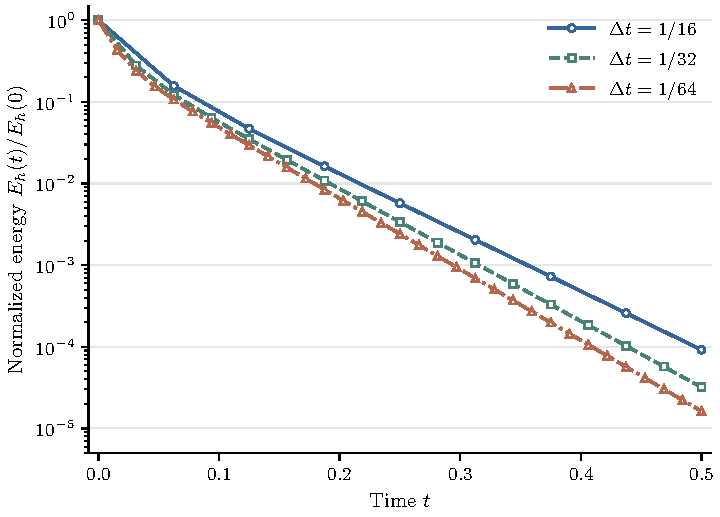
\includegraphics[width=0.70\textwidth]{figures/first_order_energy.pdf}
\caption{Normalized discrete energy for the first-order scheme in the
unforced relaxation test, $K=8$ and $T=0.5$.
The vertical axis is logarithmic. Symbols represent all computed time
levels; connecting lines are not fitted or smoothed curves.
The same discrete initial state is used for all three time steps.}
\label{fig:first-order-energy}
\end{figure}
\FloatBarrier

\subsubsection{Second-order scheme}
\label{subsec:second-order-energy}
\Cref{fig:second-order-energy} shows monotone energy decay for all
three time steps, with initial energy approximately
$4.295033\times10^{-2}$.
\Cref{tab:second-order-energy} reports the final ratios and balance
diagnostics; the largest normalized balance defect is
$3.71\times10^{-11}$.
The coarsest time step produces slower late-time decay, which is
retained in the plot. Energy dissipation therefore should not be
interpreted as evidence that the temporal error is negligible.
Since the two schemes also use different spatial approximation
orders, these figures are separate stability tests rather than
a controlled comparison of temporal accuracy. The computations
provide numerical evidence of the discrete dissipation mechanism
at the tested step sizes, not a proof for arbitrary step sizes.

\begin{table}[htbp]
\centering
\caption{Second-order unforced energy test: $K=8$, $T=0.5$.}
\label{tab:second-order-energy}
\small
\begin{tabular}{crr}
\toprule
$\dt$ & $E_h(T)/E_h(0)$ & $\max_n\epsilon_{\rm bal}^n$\\
\midrule
$1/16$ & $1.1117\times10^{-4}$ & $3.71\times10^{-11}$\\
$1/32$ & $2.5984\times10^{-5}$ & $7.77\times10^{-13}$\\
$1/64$ & $1.0438\times10^{-5}$ & $2.67\times10^{-13}$\\
\bottomrule
\end{tabular}
\end{table}

\begin{figure}[htbp]
\centering
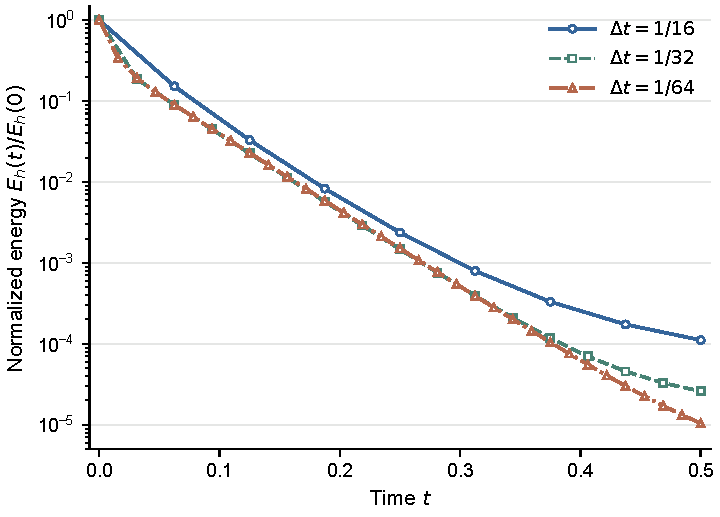
\includegraphics[width=0.70\textwidth]{figures/second_order_energy.pdf}
\caption{Normalized discrete energy for the second-order scheme in the
unforced relaxation test, $K=8$ and $T=0.5$.
The logarithmic vertical scale matches \Cref{fig:first-order-energy}.
Symbols represent all computed time levels without smoothing.
The same discrete initial state is used for all three time steps.}
\label{fig:second-order-energy}
\end{figure}
\FloatBarrier

\FloatBarrier

\subsection{Magnetically forced flow in a straight channel}
\label{subsec:straight-channel}
We next apply the second-order scheme and the five-block Algorithm~3
to three-dimensional ferrofluid transport with prescribed inflow.
The configuration is motivated by the channel-pumping examples of
Dong et al.~\cite{DongHuangHuangYang2026}, while retaining the magnetic
diffusion, compatible finite element spaces, and midpoint/extrapolation
scheme of the present work. The parameters and driving waveform below
define our computational example; they are not a reproduction of all
the parameters in that reference. All quantities are dimensionless.

\paragraph{Domain, material parameters, and initial data.}
The straight channel is
\[
  \Omega_c=(0,1)\times(0,0.2)\times(0,0.2).
\]
We denote the inlet $x=0$, outlet $x=1$, and remaining solid walls by
$\Gamma_i$, $\Gamma_o$, and $\Gamma_w$, respectively.
The material parameters, also used in the stepped channel below, are
\begin{equation}\label{eq:channel-material-parameters}
\begin{gathered}
 \rho=\mu_0=\chi_0=1,\qquad
 \kappa=\zeta=0.01,\qquad \eta=0.02,\\
 \eta^{\prime}=\lambda^{\prime}=0.001,\qquad
 \tau=0.1,\qquad \sigma=0.005.
\end{gathered}
\end{equation}
The body sources are $\bs f=\bs g=\bs r=\bs0$.
The initial velocity, angular velocity, magnetization, and magnetic
potential are zero, as are the pressure and auxiliary variables.
These data are compatible with the initially vanishing inlet and
magnetic forcing.

\paragraph{Inlet and magnetic forcing.}
Introduce the smooth ramp
\begin{equation}\label{eq:channel-ramp}
 R(s)=\begin{cases}
 0,&s\leq0,\\
 10s^3-15s^4+6s^5,&0<s<1,\\
 1,&s\geq1.
 \end{cases}
\end{equation}
The inlet profile is
\begin{equation}\label{eq:channel-inlet}
 \bs u_D=\bigl(0.25R(t/0.4)\,16Y(1-Y)Z(1-Z),0,0\bigr)^{\intercal},
 \qquad Y=\frac{y}{0.2},\quad Z=\frac{z}{0.2}.
\end{equation}
It vanishes at the inlet edges and is imposed by nodal interpolation
and finite element Dirichlet lifting.

Eight dipoles are placed outside the channel at
\[
 \bs x_i^-=(0.2i,-0.15,0.1),\qquad
 \bs x_i^+=(0.2i,0.35,0.1),\qquad i=1,\ldots,4,
\]
with directions $\bs d_i^-=(0,1,0)^{\intercal}$ and
$\bs d_i^+=(0,-1,0)^{\intercal}$.
We prescribe
\begin{align}
 \Phi_a(\bs x,t)
 &=\sum_{i=1}^4 a_i(t)
   \sum_{\epsilon\in\{-,+\}}
   \frac{\bs d_i^{\epsilon}\cdot(\bs x_i^{\epsilon}-\bs x)}
   {|\bs x_i^{\epsilon}-\bs x|^3},
 &\bs h_a&=\nabla\Phi_a,\label{eq:channel-dipoles}\\
 a_i(t)
 &=C_a A R\!\left(\frac{t-0.2}{0.4}\right)
 \left[0.7+0.3\cos\!\left(2\pi\left(t-\frac{0.2i}{0.8}\right)\right)\right],
 &C_a&=3\times10^{-4}.\label{eq:channel-pulse}
\end{align}
The dipole positions are fixed; the phase shifts act on their
time-dependent strengths. The magnetic forcing has period one after
the ramp. We take $A=1$ for the magnetic case and $A=0$ for a
zero-field control with the same inlet data.
In the notation of the model, $\bs H_e=-\mu_0\bs h_a$.
Since all sources lie outside the fluid, $\Phi_a$ is harmonic there.
Consequently, the magnetic-potential load is
\[
 (\bs G_e,\nabla\psi_h),\qquad
 \bs G_e=\mu_0\partial_t\bs h_a
       +\frac{\mu_0+\chi_0}{\tau}\bs h_a.
\]

\paragraph{Open-boundary formulation.}
We impose $\bs u=\bs0$ on $\Gamma_w$ and the gradient-traction condition
\begin{equation}\label{eq:channel-outlet}
 \bigl((\eta+\zeta)\nabla\bs u-pI\bigr)\bs n=\bs0
 \qquad\text{on }\Gamma_o,
\end{equation}
where $p$ is the physical pressure and the computed pressure slot is
$\widetilde p=p-\mu_0\bs m\cdot\bs H/2$.
The outlet fixes the pressure level, so no pressure-mean constraint is
added in these open-channel runs. On the entire boundary we prescribe
\begin{equation}\label{eq:channel-magnetic-boundary}
\begin{gathered}
 \bs\omega=\bs0,\qquad \bs m\cdot\bs n=0,\qquad
 \bs k\times\bs n=\bs0,\\
 (\bs H+\bs m)\cdot\bs n=\bs h_a\cdot\bs n,
 \qquad \int_{\Omega_c}\varphi_h\,\mathrm dx=0.
\end{gathered}
\end{equation}
The tangential trace of $\bs z_h$ is zero on $\Gamma_w$ and free
on the inlet and outlet. The trace of $\varpi_h$ is zero on
$\Gamma_i\cup\Gamma_w$ and free on $\Gamma_o$.
The weak definition of $\vartheta_h$ includes the prescribed normal load:
\[
 (\vartheta_h,v_h)
 =(\nabla\varphi_h,\nabla v_h)
   -\langle\bs h_a\cdot\bs n,v_h\rangle_{\partial\Omega_c}.
\]

The nine volume equations and their five-block coupling are retained.
The open-boundary extension includes the term
$\frac{\mu_0}{2}(\curl\bs z_h,\nabla\psi_h)$ in the
magnetic-potential equation. To implement \eqref{eq:channel-outlet}
with the gradient/curl form of the momentum equation, its residual
also contains
\begin{equation}\label{eq:channel-outlet-residual}
\begin{aligned}
 \mathcal R_{\Gamma_o}(\bs v_h)
 &=-\langle\bs t_\Delta,\bs v_h\rangle_{\Gamma_o}
 +\frac{\rho}{2}\langle(\bs u_*\cdot\bs n)\bs u,\bs v_h\rangle_{\Gamma_o},\\
 \bs t_\Delta
 &=-\zeta(\nabla\bs u)^{\intercal}\bs n+2\zeta\bs n\times\bs\omega\\
 &\quad+\frac{\mu_0}{2}\bigl[(\bs m_*\cdot\bs H)\bs n
       +\bs n\times(\bs H\times\bs m_*)\bigr].
\end{aligned}
\end{equation}
Here the unstarred fields in the evolution residuals are midpoint
values, while stars denote the prescribed nonlinear-startup or
extrapolated coefficients. The inlet lifting and the normal load in
the $\vartheta_h$ relation use endpoint data.
These boundary conditions extend the homogeneous setting of the
analysis. The closed-boundary energy estimates are not asserted for
this driven open-boundary problem.

\paragraph{Discretization and results.}
We use the second-order finite element spaces of
\Cref{subsec:experiment-setup}, $\dt=0.005$, and $T=2$.
The initial step solves the nonlinear midpoint equations; subsequent
steps use the specified extrapolation and Algorithm~3, including
the fifth-block feedback. Assembly uses quadrature degree eight.
The Schur solves use relative and absolute tolerances $10^{-11}$
and $10^{-16}$; the nonlinear startup uses relative tolerance
$10^{-9}$ with an absolute residual floor of $10^{-14}$.
The channel meshes contain $30K^3$ tetrahedra, obtained from a
$5K\times K\times K$ Cartesian partition.
The magnetic runs use $K=4,8,12$, and the control uses $K=12$.

\Cref{fig:channel-u,fig:channel-m,fig:channel-omega} show the
$K=12$ magnetic solution at $t=2$.
The velocity retains a predominantly axial profile, whereas the
magnetization has a nonuniform distribution set by the dipole field
and its coupled response. The particle angular velocity is appreciable
in the sheared portions of the flow; it is distinct from the fluid
vorticity $\curl\bs u_h$.

At $T=2$, native volume-$L^2$ differences between the $K=8$ and
$K=12$ solutions, normalized by the $K=12$ norm, are
\begin{center}
\begin{tabular}{lrrrr}
\toprule
Field & $\bs u$ & $\bs m$ & $\bs\omega$ & $\bs H$\\
\midrule
Relative difference (\%) & 0.13524 & 3.29718 & 0.71893 & 3.14611\\
\bottomrule
\end{tabular}
\end{center}
These are adjacent-mesh differences, not errors against an exact
solution. They were integrated on a common refinement and checked
with quadrature degrees four and six.
The same-mesh zero-field control has zero magnetization and magnetic
field. Its differences from the magnetic run are $0.00725\%$ in
velocity and $0.15803\%$ in angular velocity in the same native norm,
with the magnetic solution as denominator. These small increments
have not been independently established to be mesh-converged.
The prescribed inlet fixes the through-flow; this comparison concerns
field response under magnetic forcing and does not establish a net
magnetic pumping gain.

\begin{figure}[!htbp]
\centering
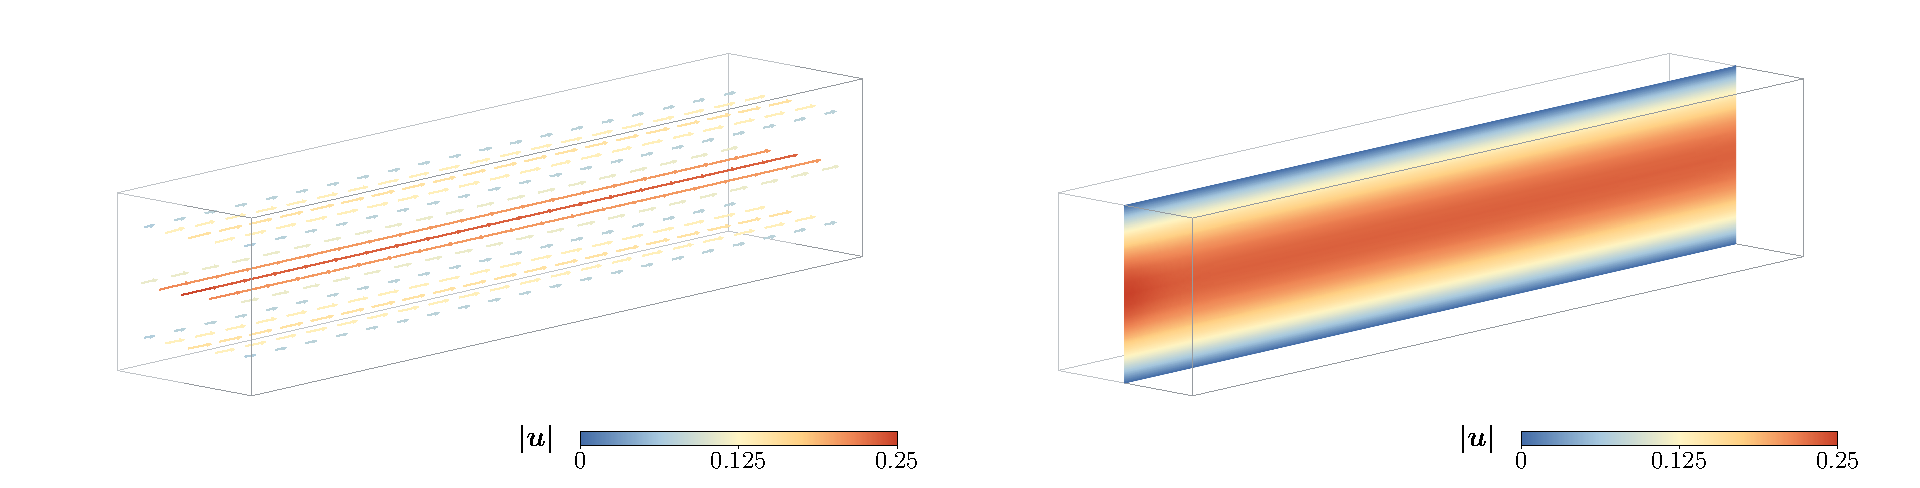
\includegraphics[width=\textwidth]{figures/applications/channel_u.pdf}
\caption{Straight-channel flow at $t=2$ on $K=12$: velocity vectors
(left) and the velocity magnitude on $z=0.1$ (right).}
\label{fig:channel-u}
\end{figure}
\begin{figure}[!htbp]
\centering
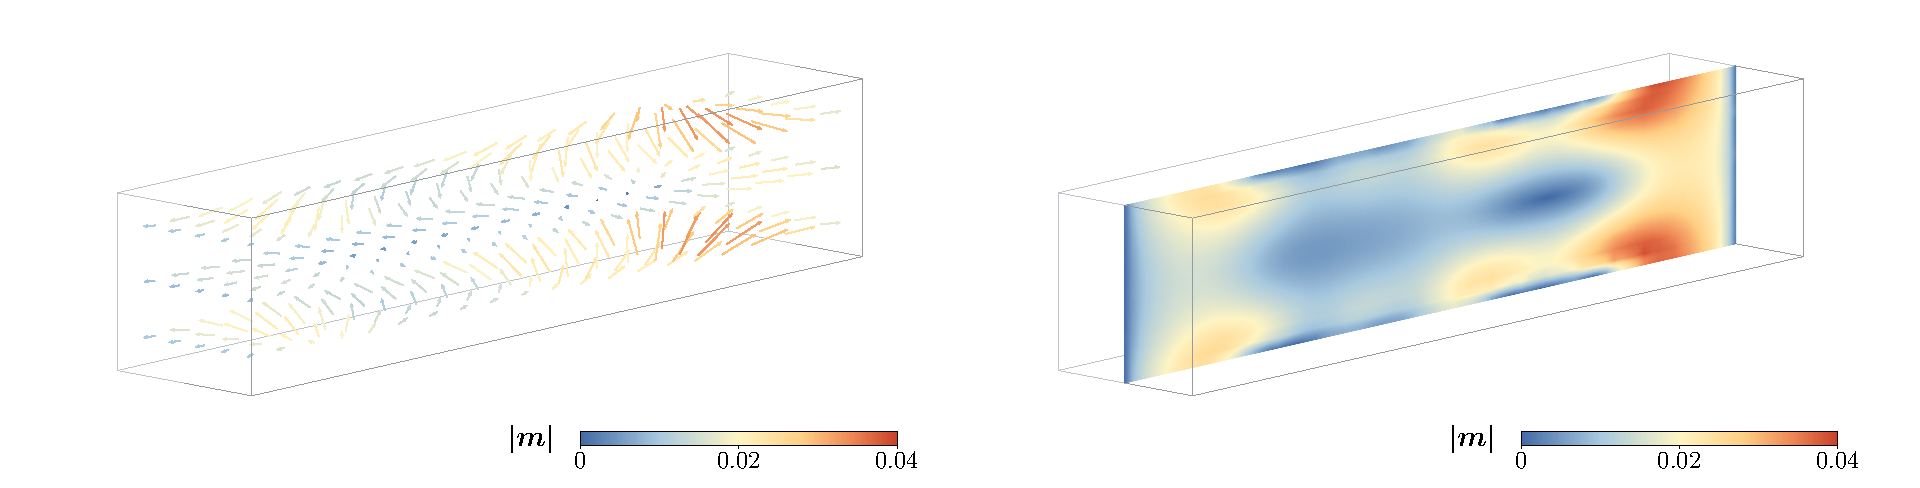
\includegraphics[width=\textwidth]{figures/applications/channel_m.pdf}
\caption{Straight-channel flow at $t=2$ on $K=12$: magnetization
vectors (left) and the magnetization magnitude on $z=0.1$ (right).}
\label{fig:channel-m}
\end{figure}
\begin{figure}[!htbp]
\centering
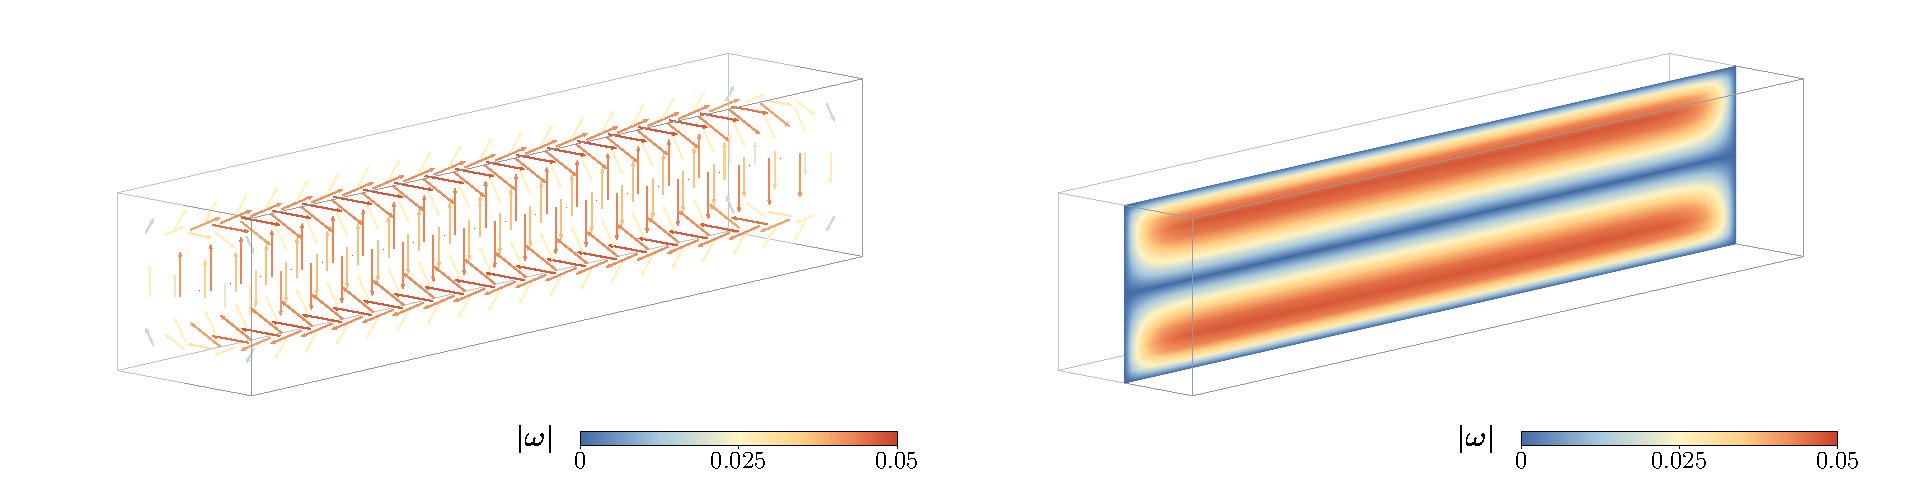
\includegraphics[width=\textwidth]{figures/applications/channel_omega.pdf}
\caption{Straight-channel flow at $t=2$ on $K=12$: particle angular
velocity vectors (left) and their magnitude on $z=0.1$ (right).
The arrows display instantaneous vectors, not particle trajectories.}
\label{fig:channel-omega}
\end{figure}
\FloatBarrier

\subsection{Magnetically forced flow over a backward-facing step}
\label{subsec:backward-facing-step}
To examine the same coupled solver in a channel with a sudden
expansion, we consider
\begin{equation}\label{eq:step-domain}
 \Omega_s=(0,1)\times(0,0.2)\times(0,0.2)
 \setminus\bigl([0,0.2]\times[0,0.2]\times[0,0.1]\bigr).
\end{equation}
The upstream bottom is raised to $z=0.1$ for $x\leq0.2$.
The fluid volume is $0.036$; the inlet $x=0$, $z>0.1$ has area
$0.02$, and the outlet $x=1$ has area $0.04$.
The vertical step face and all remaining boundary faces belong
to the no-slip wall $\Gamma_w$.
The geometry and the dipole locations follow the three-dimensional
step configuration in \cite{DongHuangHuangYang2026}.

The material parameters, zero initial data, zero body sources,
outlet traction, and magnetic and auxiliary boundary conditions are
those stated in \Cref{subsec:straight-channel}, with $\Omega_c$
replaced by $\Omega_s$. The inlet profile is
\begin{equation}\label{eq:step-inlet}
 \bs u_D=\bigl(0.25R(t/0.4)\,16Y(1-Y)Z_s(1-Z_s),0,0\bigr)^{\intercal},
 \qquad Y=\frac{y}{0.2},\quad Z_s=\frac{z-0.1}{0.1}.
\end{equation}
It is supported on the upper half of the inlet and vanishes on
its edges. The inlet and homogeneous wall values are imposed
separately, so the polynomial inlet extension is not applied to the
vertical step face. After ramp-up, the analytic inlet flux is
$1/450$, one half of the straight-channel value because the inlet
area is halved.

The applied field retains \eqref{eq:channel-dipoles}--\eqref{eq:channel-pulse},
with $A=1$, but uses
\begin{equation}\label{eq:step-dipoles}
 \bs x_i^-=(0.2i,-0.2,0.1),\qquad
 \bs x_i^+=(0.2i,0.4,0.1),\qquad i=1,\ldots,4,
 \qquad C_a=7\times10^{-4}.
\end{equation}
The directions remain $\bs d_i^{\pm}=\mp(0,1,0)^{\intercal}$,
with the upper sign corresponding to the upper row.
Thus the waveform, ramp times, period, and phase speed are unchanged,
while the magnetic-source distance and prefactor are explicitly
different. In particular, the relaxation time remains $\tau=0.1$
and the diffusion coefficient remains $\sigma=0.005$.

\paragraph{Mesh and time stepping.}
We use the same second-order spaces, nonlinear midpoint startup,
subsequent extrapolation, quadrature, and solver tolerances as in
the straight channel. The time step is $0.005$ and the simulation
runs to $T=2$.
A conforming tetrahedral mesh is formed from a $5K\times K\times K$
background partition, with the solid cells removed.
Before extracting the fluid mesh, its logical axial coordinate
$\xi$ is mapped to $x$ by the continuous piecewise affine function
specified by
\[
\begin{array}{c|ccccc}
\xi&0&0.1&0.2&0.6&1\\\hline
x&0&0.15&0.2&0.4&1.
\end{array}
\]
This grades the mesh near the step; the transverse coordinates
remain uniform. The resulting mesh has $27K^3$ tetrahedra.
The following visualizations use $K=4$, namely $1728$ tetrahedra.

\paragraph{Field visualization and interpretation.}
\Cref{fig:step-u,fig:step-m,fig:step-omega} use the actual saved
time layer $t=0.715$ (step $143$), rather than a temporally
interpolated state. All three fields use this same time.
The velocity spreads into the larger downstream cross-section after
the step. The magnetization exhibits spatially varying direction
and magnitude, while the angular-velocity distribution is influenced
by the shear near the step and the channel walls.
The displayed angular velocity is the particle spin.

The right panels show the full three-component magnitude on $y=0.1$.
The magnetization arrows are sampled on that same plane; the velocity
and angular-velocity arrows use sparse three-dimensional locations.
Solid-region samples are excluded. The linear arrow scaling and the
color scales are fixed over the stored time interval.
Point values come from the original finite element fields without
RT vertex averaging; interpolation in the filled color surface is
used only for display, not for evaluating finite element norms.
The color limits for $\bs u$, $\bs m$, and $\bs\omega$ are
$0.25$, $0.04$, and $0.04$, respectively.

The $400$-step $K=4$ trajectory passed the stated algebraic and
boundary checks: its maximum recomputed relative residual was
$2.03\times10^{-10}$, and its largest recorded relative inlet--outlet
flux imbalance was $1.12\times10^{-14}$.
A full-interval $K=4$ comparison with $\dt=0.0025$ gave endpoint
relative native volume-$L^2$ differences below $2.9\times10^{-5}$ for
$\bs u$, $\bs m$, $\bs\omega$, and $\bs H$.
These checks assess the implementation and time-step sensitivity.
At the displayed spatial resolution, the figures are a qualitative
illustration; quantitative mesh independence of the step-flow
observables remains to be assessed. In particular, no resolved
reattachment length, corner extremum, or magnetic pumping efficiency
is inferred from these plots. The nonconvex geometry and open
boundary conditions also lie outside the homogeneous convex-domain
setting used in the analysis.

\begin{figure}[!htbp]
\centering
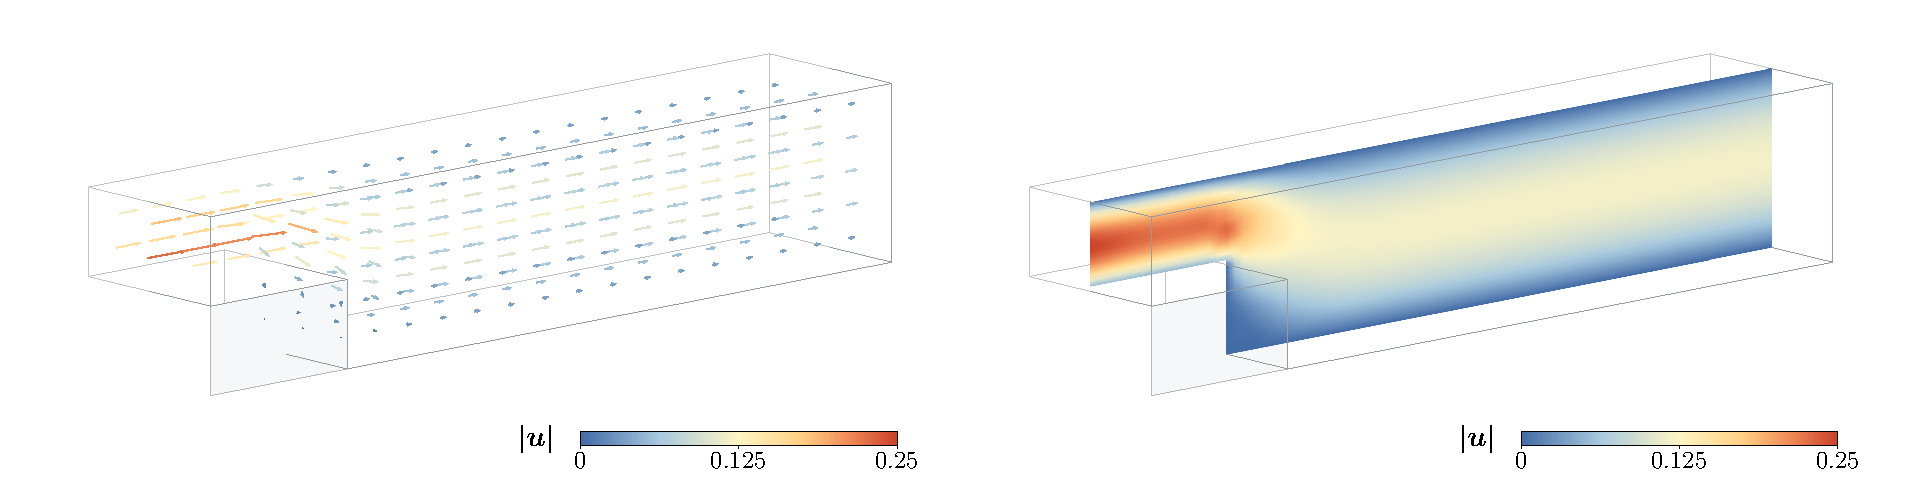
\includegraphics[width=\textwidth]{figures/applications/step_u.pdf}
\caption{Backward-facing-step flow at $t=0.715$ on $K=4$:
velocity vectors (left) and the velocity magnitude on $y=0.1$
(right). The unfilled upstream region is the solid step.}
\label{fig:step-u}
\end{figure}
\begin{figure}[!htbp]
\centering
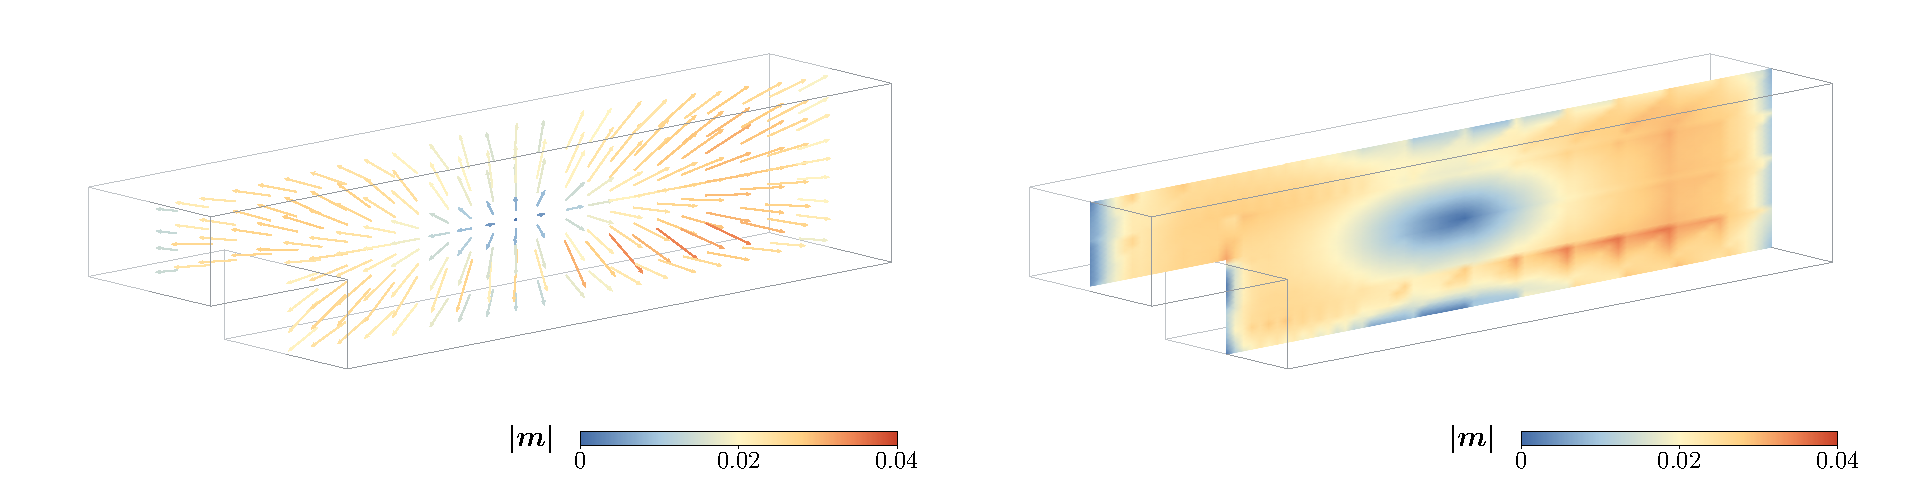
\includegraphics[width=\textwidth]{figures/applications/step_m.pdf}
\caption{Backward-facing-step flow at $t=0.715$ on $K=4$:
magnetization vectors (left) and their full magnitude (right),
both sampled on $y=0.1$.}
\label{fig:step-m}
\end{figure}
\begin{figure}[!htbp]
\centering
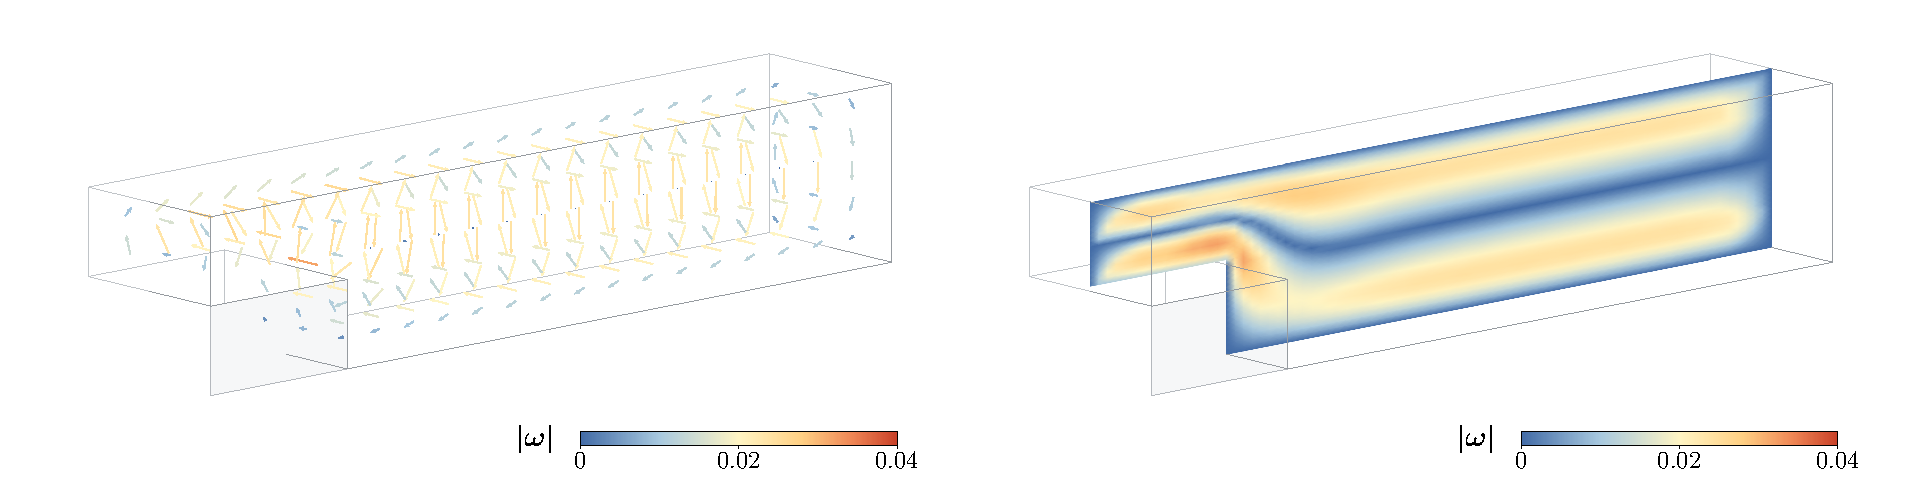
\includegraphics[width=\textwidth]{figures/applications/step_omega.pdf}
\caption{Backward-facing-step flow at $t=0.715$ on $K=4$:
particle angular velocity vectors (left) and their magnitude
on $y=0.1$ (right).}
\label{fig:step-omega}
\end{figure}
\FloatBarrier


\begin{thebibliography}{1}
\bibitem{Barattafenics}
I.~A. Baratta, J.~P. Dean, J.~S. Dokken, M. Habera, J.~S. Hale,
C.~N. Richardson, M.~E. Rognes, M.~W. Scroggs, N. Sime, and G.~N. Wells,
DOLFINx: The next generation FEniCS problem solving environment, 2023.
\bibitem{DongHuangHuangYang2026}
X.~Dong, H.~Huang, Y.~Huang, and X.~Yang,
A fully discrete finite element method with second-order temporal
accuracy for the Rosensweig model,
\emph{J. Comput. Phys.}, 549 (2026), 114617.
\end{thebibliography}
\end{document}
